% ============================ Enrico Ribiani 16-03-2021 ====================================================================
% Base per i documenti  
\documentclass[12pt]{article}
% ------------ pacchetti necessari ----------------
\usepackage[a4paper, total={6in, 8in},margin=1in]{geometry} % formattazione decente della pagina
\usepackage{graphicx}                            % need for figure
\usepackage{amsmath}
\usepackage{amsfonts}                            % if you want the fonts
\usepackage{amssymb}                             % if you want extra symbols
\usepackage{graphicx}  
\renewcommand{\figurename}{Figura}  
\renewcommand{\contentsname}{Indice}                        % need for figures
\usepackage{mathptmx}
\usepackage{float}                               % serve per mettere tabelle e immagini dove si vuole 
\usepackage[utf8]{inputenc}
\usepackage{textcomp}
\usepackage[hang,flushmargin,bottom]{footmisc}   % footnote format
\usepackage{fancyhdr, lastpage}
\usepackage{titlesec}
\usepackage[table,dvipsnames]{xcolor}
%\pagestyle{fancy}
%\renewcommand{\headrulewidth}{0pt}
%\renewcommand*\contentsname{Indice}
\titleformat{\section}{\normalsize\bfseries}{\thesection.}{1em}{}	% required for heading numbering style
\titleformat*{\section}{\Large\bfseries}
\titleformat*{\subsection}{\large\bfseries}
%\usepackage{siunitx}
%\usepackage{tikz}
\usepackage{circuitikz}
%\usepackage[siunitx]{circuitikz}
\usepackage{multirow}
\usepackage{tikz}
\usepackage{amsmath}
\usepackage{shorttoc}
\usetikzlibrary{angles,quotes}
\usepackage{placeins}

\usepackage{wasysym}
%===================links=================
\usepackage{hyperref}
\hypersetup{
    colorlinks=true,
    linkcolor=darkgray,
    filecolor=Green,      
    urlcolor=Cyan,
    pdftitle={SAMPLE},
    pdfpagemode=FullScreen,
    }
%===================inizio pagina del titolo=================
\begin{document}
\begin{titlepage}
	\begin{center}
		% ------------------ inizio immagine logo ----------
		\begin{figure}
			\centering
			
\includegraphics[scale=1.2]{logo.png}
			\label{fig:logo}
		\end{figure}
		% ------------------ fine immagine logo ----------
		% ------------------ fine immagine logo ----------
		-------------------------------------------------------------------------------------\\
		\vspace{2\baselineskip}
		\large Enrico Ribiani\\
		\large 5AUB\\
		\vfill

		\Huge{\textbf{Macchina per foratura}}\\
		\vfill

		\LARGE{Relazione n°3}\\
		\vfill
		\large{24-02-2023}
	\end{center}
	%=============== fine pagina titolo ===============
\end{titlepage}
\thispagestyle{empty}
\tableofcontents

\newpage
\setcounter{page}{1}
\section{Introduzione}
In questa esercitazione laboratoriale è stata richiesta la gestione completa di una macchina automatica con il compito di forare e immagazzinare dei pezzi.\\
La macchina è di tipo pneumatico infatti il suo principio di funzionamento è basato su tre cilindri pneumatici a doppio effetto, il nostro incarico è quello di progettare e programmare il sistema di controllo e di potenza segliendo le valvole più idonee alla soluzione da noi utilizzata.
\subsection{Soluzione da noi utilizzata}
Per comandare i cilindri abbiamo scelto di utilizzare tre valvole \textit{5/2} con azionamento elettrico in apertura e chiusura, poichè rappresentano la soluzione più efficente e semplice per azionare un cilindro a doppio effetto tramite un plc.\\
\noindent
Abbiamo scelto di gestire il ciclo tramite un plc programmato con il linguaggio a contatti ladder, questa soluzione è stata simulata in laboratorio
tramite il programma \textit{PneumaticStudio}.\\
\begin{figure}[!h]
	\centering
	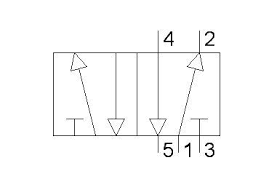
\includegraphics[scale=0.4]{52.png}
	\caption{Valvola 5/2}
	\label{fig:5/2}
\end{figure}

\section{Funzionamento}
\begin{figure}[h]
	\centering
	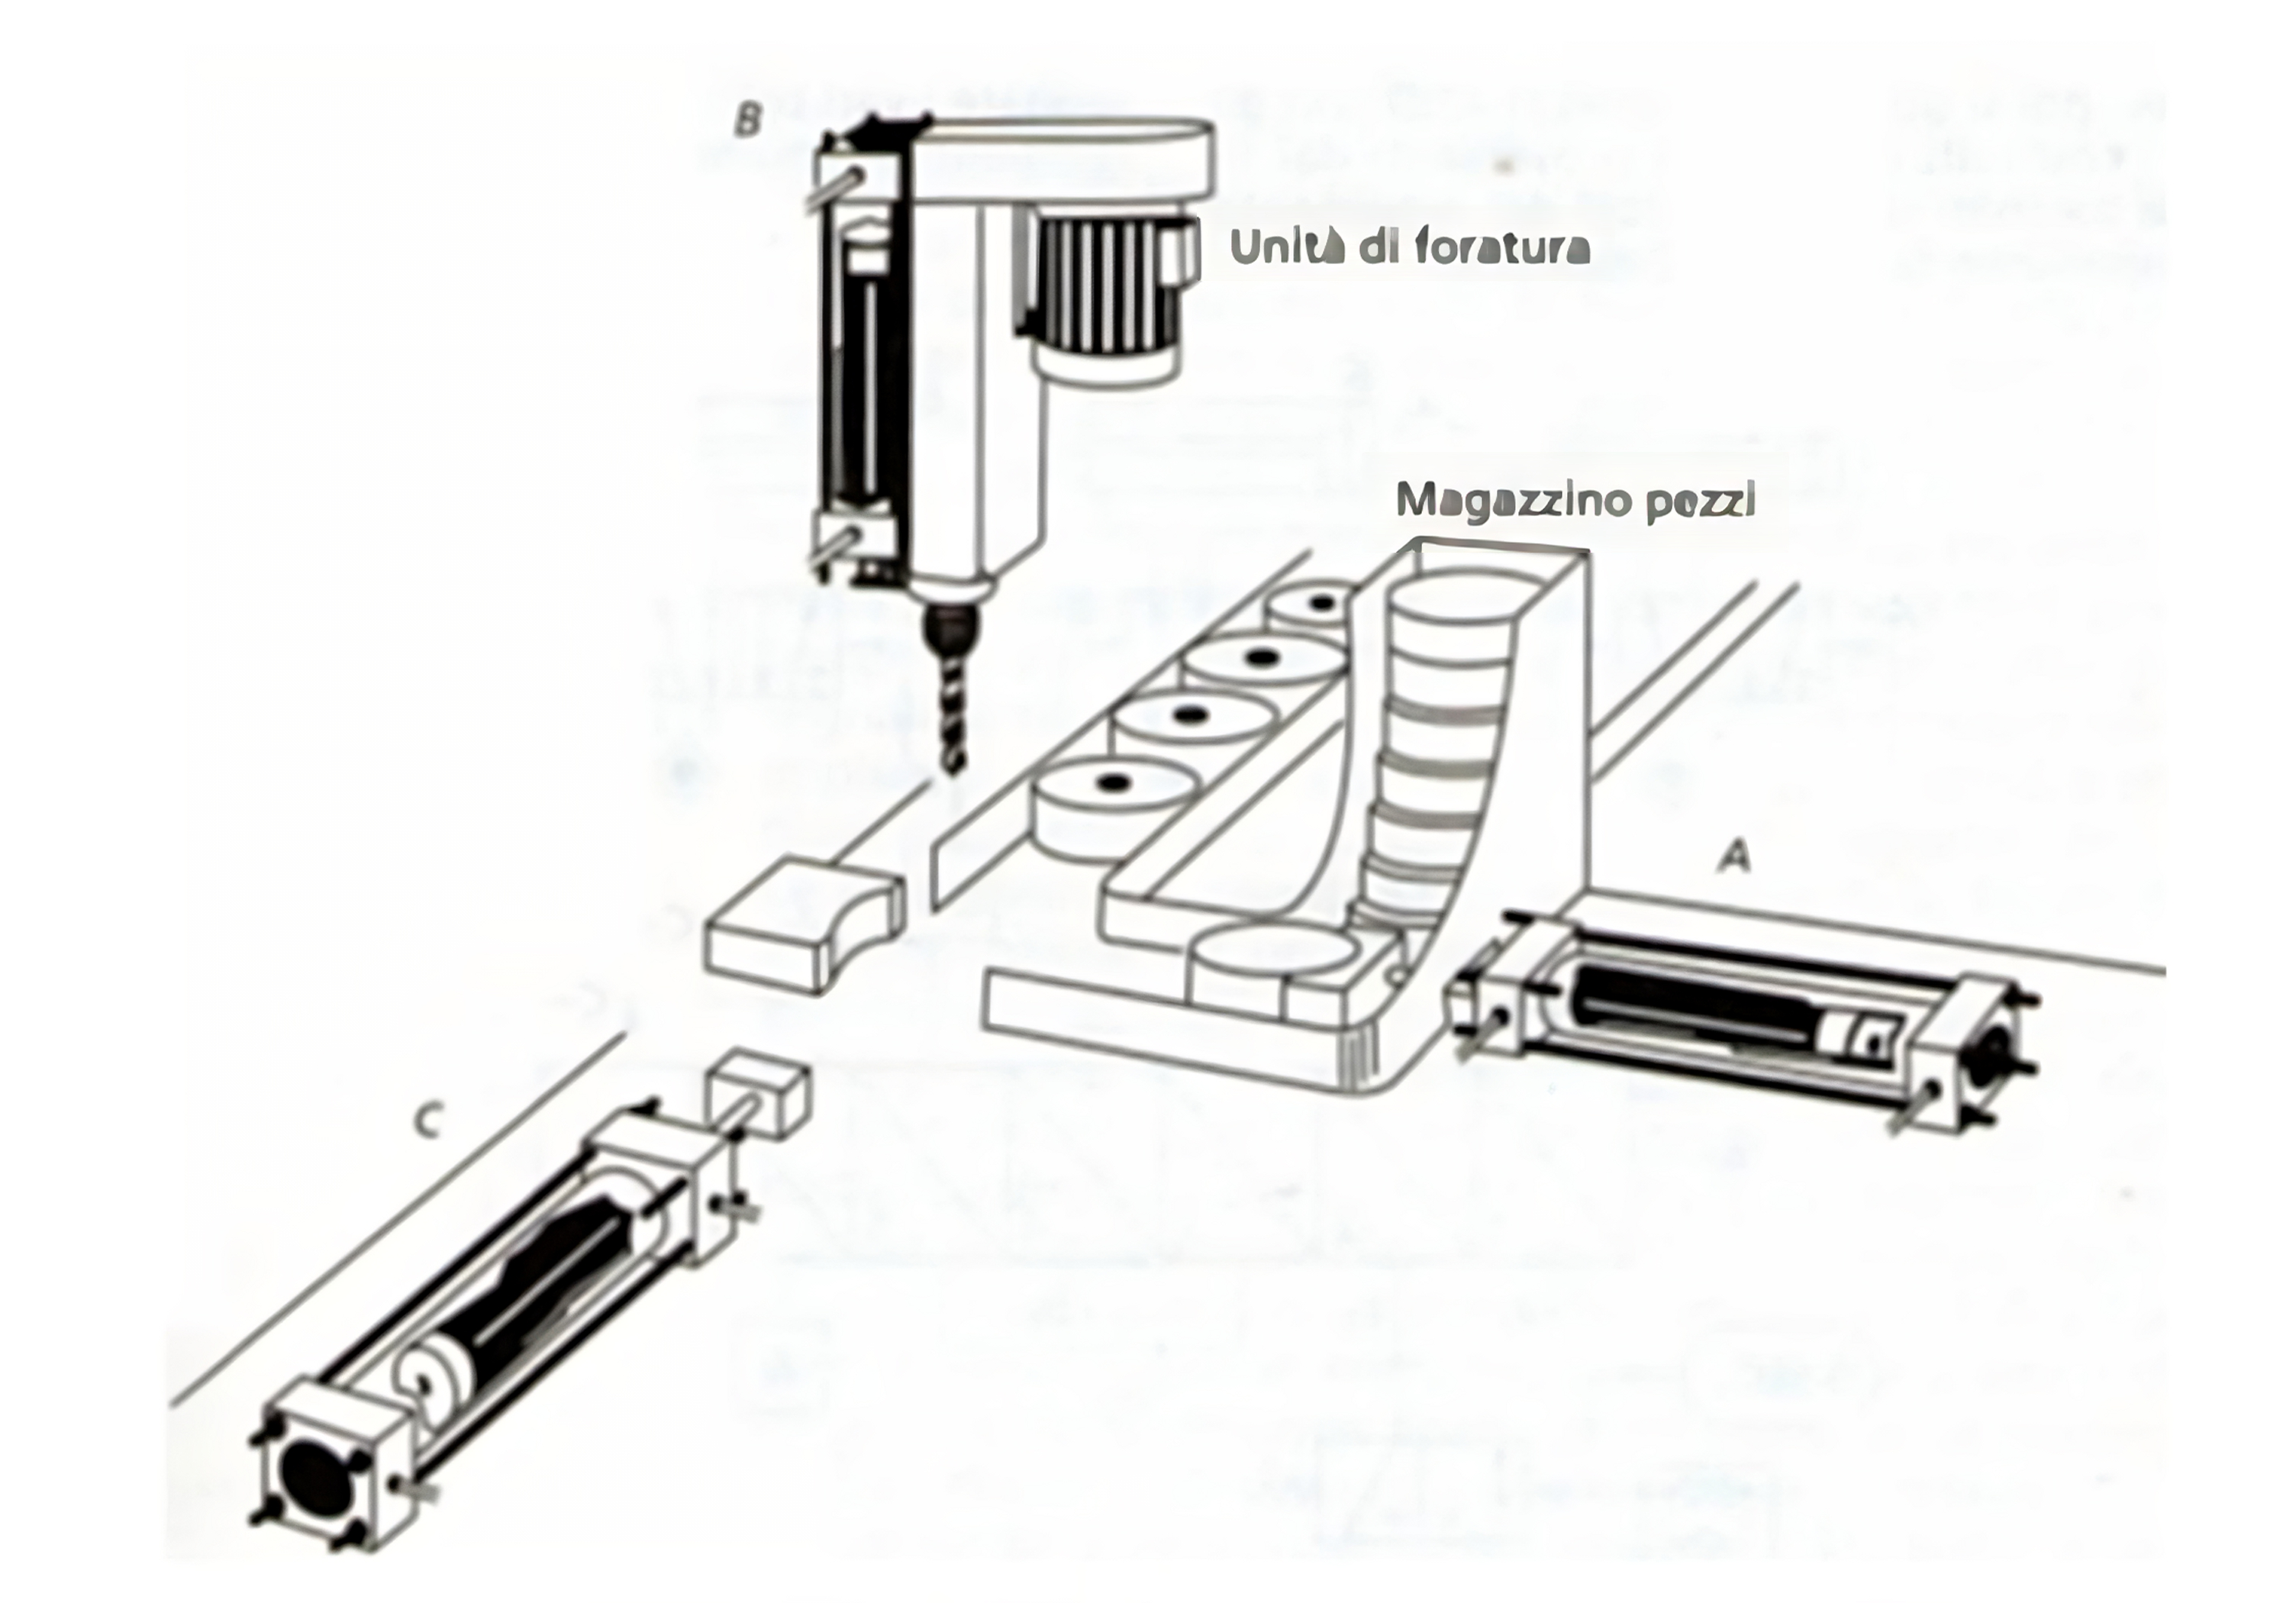
\includegraphics[scale=0.05]{schema-macchina.png}
\end{figure}
\noindent
La macchina inizia a lavorare alla pressione del pulsante di start, dopodichè il cilindro \textbf{A} ossia quello incaricato di posionare e
bloccare i pezzi sotto al trapano a colonna si estrae.\\
Una volta estrato completamente rimane in posizione e il cilindro \textbf{B} si estrae forando tramite il trapano attaccato a esso il pezzo,
una volta estratto completamente il pezzo sarà forato e quindi si ritrarrà.\\
Con il cilindro B ritratto il cilindro A tornerà alla posizione iniziale in modo da consentire al cilindro \textbf{C} di spingere nel
magazzino il pezzo forato.\\
Queste due ultime azioni avvengono contemporaneamente.\\
\subsection{Diagramma funzionale}
\begin{figure}[!h]
	\centering
	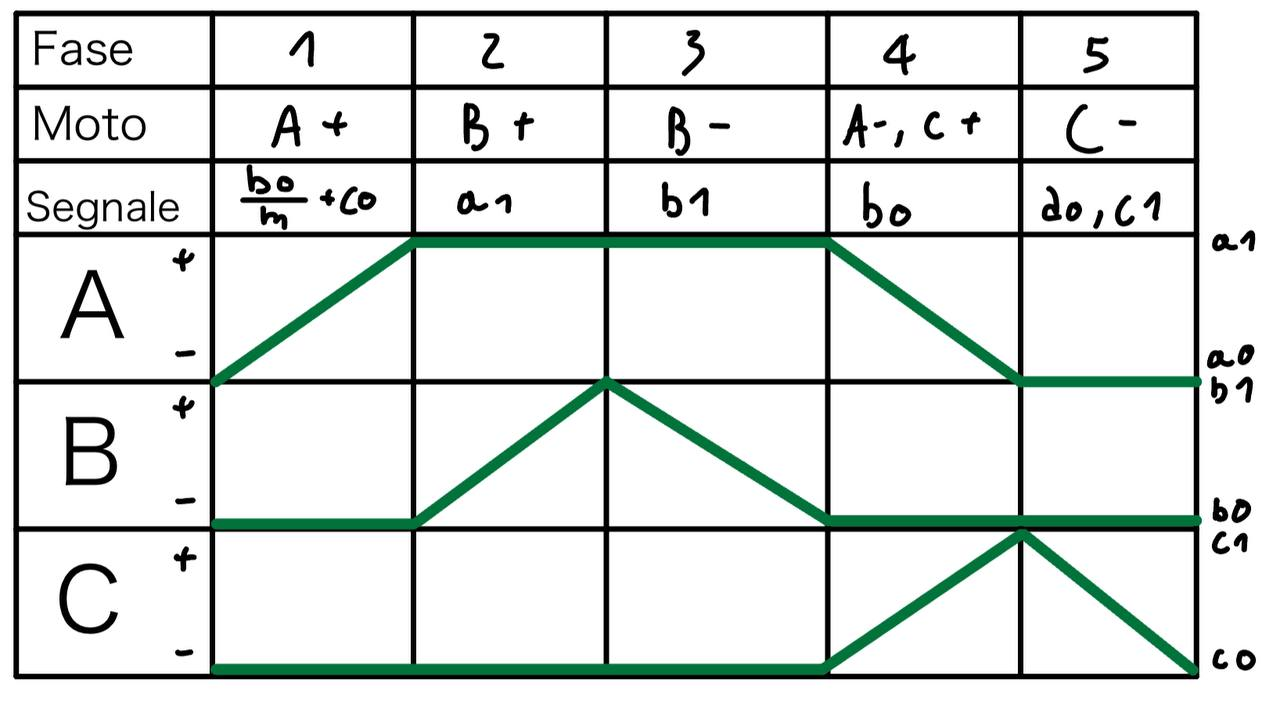
\includegraphics[scale=0.2]{sfunzionale.jpg}
	%\caption{Caption}
	%\label{fig:my_label}
\end{figure}
\section{Componenti}
\subsubsection{Cilindro}
È stato scelto il cilindro \textit{DSBC 2102632} prodotto da Festo poichè rappresenta uno standard per i cilindri a
doppio effetto, ne vengono prodotti di molte dimensioni (1-2800 mm), rispettano la norma ISO15552 e sono fornite di dichiarazione di conformità
oltre che il marchio CE \\
\subsubsection{Valvole}
Per controllare questo cilindro scelto la casa produttrice consiglia la valvola universale \textit{VUVS-LK20-B52-D-G18-1C1-S} con funzione 5/2 e azionamento elettrico
con il controllo standardizzato a 24V.\\
Il prodotto presenta dichiarazione di conformità e marchio CE.\\
\subsubsection{Finecorsa}
Tramite il configuratore Festo andiamo a scegliere i sensori di finecorsa \textit{SMT-8M-A-PS-24V-E-2,5-OE} che rispettano lo standard
EN 60947-5-2 funzionanti a 24V e quindi compatibili con lo standard infine il tubo \textit{PEN-8X1,25-BL} con cui collegare cilindri e
valvole.\\
Il prodotto presenta dichiarazione di conformità e marchio CE.\\
\subsubsection{Plc}
Per la scelta del plc i parametri da rispettare sono la tensione di funzionamento standard 24V e la disposizione di almeno 7 ingressi e
10 uscite.\\
Il plc Schneider Electric \textit{TM241CEC24T} risulta idoneo, ma visto che sarà a programmato tramite il
linguaggio ladder si può utilizzare il plc Zelio logic\textit{SR3B261BD}.\\
Tutti i prodotti presentano dichiarazione di conformità e marchio CE.\\
\subsection{Preventivo}
\begin{table}[H]
	\centering
	\begin{tabular}{|c|c|c|c|c|} \hline
		\rowcolor{ForestGreen!70} Codice prodotto            & Dispositivo & Quantità & Prezzo & Totale \\
		\hline
		\rowcolor{SpringGreen!80} DSBC 2102632               & cilindro    & 3        & 190    & 570    \\
		\hline
		\rowcolor{LimeGreen!80}   VUVS-LK20-B52-D-G18-1C1-S  & valvola 5/2 & 3        & 70     & 210    \\
		\hline
		\rowcolor{SpringGreen!80}   SR3B261BD                & plc         & 1        & 300    & 300    \\
		\hline
		\rowcolor{LimeGreen!80} PEN-8X1,25-BL                & tubo        & 1        & 40     & 40     \\
		\hline
		\rowcolor{SpringGreen!80}   SMT-8M-A-PS-24V-E-2,5-OE & finecorsa   & 6        & 30     & 180    \\
		\hline
		\rowcolor{LimeGreen!80} 82-5551.1133L                & pulsante NO & 1        & 20     & 20     \\
		\hline
		\hline
		\rowcolor{LimeGreen!40}                              &             &          &        & 1320   \\
		\hline
	\end{tabular}
\end{table}
Prezzi compresi di IVA.\\
\newpage
\section{Allegati}
\subsection{Norme di riferimento}
ISO15552 - Normativa sui cilindri pneumatici\\
ISO8573  - Normativa sull'aria compressa e il filtraggio\\
CEI 3-34 - Nomenclatura\\
IEC 1131-3 - Normativa linguaggi PLC\\
IEC 947.4.1 - CEI EN 60947.41 - Apparecchiature in bassa tensione \\
\subsubsection{Tabella Input/Output}
\begin{table}[H]
	\centering
	\begin{tabular}{|c|c|c|} \hline
		\rowcolor{Blue!80}  Sigla Input     & Componente  & Ingresso \\
		\hline
		\rowcolor{LimeGreen!50}  a0    & FC A-       & I1       \\
		\hline
		\rowcolor{Green!50}    a1       & FC A+       & I2       \\
		\hline
		\rowcolor{LimeGreen!50}  b0    & FC B-       & I3       \\
		\hline
		\rowcolor{Green!50}    b1       & FC B+       & I4       \\
		\hline
		\rowcolor{LimeGreen!50}  c0    & FC C-       & I5       \\
		\hline
		\rowcolor{Green!50}    c1       & FC C+       & I6       \\
		\hline
		\rowcolor{LimeGreen!50}  start & pulsante NO & I7       \\
		\hline
	\end{tabular}
	\caption{Tabella Input}
\end{table}

\begin{table}[H]
	\centering
	\begin{tabular}{|c|c|c|} \hline
		\rowcolor{Blue!80}  Sigla Output    & Componente       & Uscita \\
		\hline
		\rowcolor{LimeGreen!50}  A\_dx & pos. A valvola 1 & Q2     \\
		\hline
		\rowcolor{Green!50}    A\_sx    & pos. B valvola 1 & Q1     \\
		\hline
		\rowcolor{LimeGreen!50}  B\_dx & pos. A valvola 2 & Q4     \\
		\hline
		\rowcolor{Green!50}    B\_sx    & pos. B valvola 2 & Q3     \\
		\hline
		\rowcolor{LimeGreen!50}  C\_dx & pos. A valvola 3 & Q6     \\
		\hline
		\rowcolor{Green!50}    C\_sx    & pos. B valvola 3 & Q5     \\
		\hline
	\end{tabular}
	\caption{Tabella Output}
\end{table}
\newpage
\subsection{PneumaticStudio}
\begin{figure}[h]
	\centering
	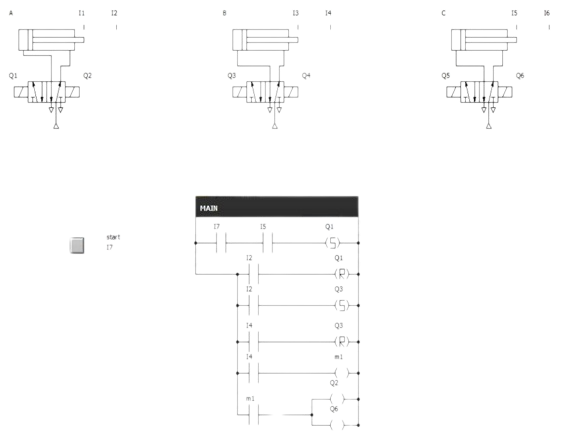
\includegraphics[scale=0.9]{ps.png}
	\label{fig:pneumatic studio}
\end{figure}
\newpage


\end{document}